\documentclass[tikz,border=3mm]{standalone}
\usepackage{tikz}
\usetikzlibrary{angles,quotes,calc,intersections}
\begin{document}
% TikZ 1
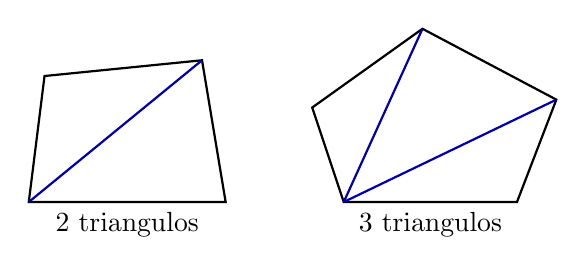
\begin{tikzpicture}[scale=1]
\coordinate (A) at (0,0); \coordinate (B) at (2.5,0); \coordinate (C) at (2.2,1.8); \coordinate (D) at (.2,1.6);
\draw[thick] (A)--(B)--(C)--(D)--cycle;
\draw[blue!70!black,thick] (A)--(C);
\node[below] at (1.25,0) {2 triangulos};
\coordinate (E) at (4,0); \coordinate (F) at (6.2,0); \coordinate (G) at (6.7,1.3); \coordinate (H) at (5,2.2); \coordinate (I) at (3.6,1.2);
\draw[thick] (E)--(F)--(G)--(H)--(I)--cycle;
\draw[blue!70!black,thick] (E)--(G);
\draw[blue!70!black,thick] (E)--(H);
\node[below] at (5.1,0) {3 triangulos};
\end{tikzpicture}
\hspace{1cm}
% TikZ 2
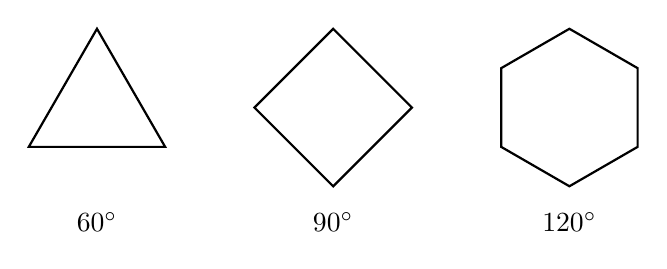
\begin{tikzpicture}[scale=1]
\foreach \n/\x/\name in {3/0/60^{\circ},4/3/90^{\circ},6/6/120^{\circ}}{
  \begin{scope}[shift={(\x,0)}]
  \foreach \k in {1,...,\n}{\coordinate (P\k) at ({90+360/\n*(\k-1)}:1);}
  \draw[thick] (P1) \foreach \k in {2,...,\n}{--(P\k)} --cycle;
  \end{scope}
  \node at (\x,-1.45) {$\name$};
}
\end{tikzpicture}

\vspace{1cm}

% TikZ 3
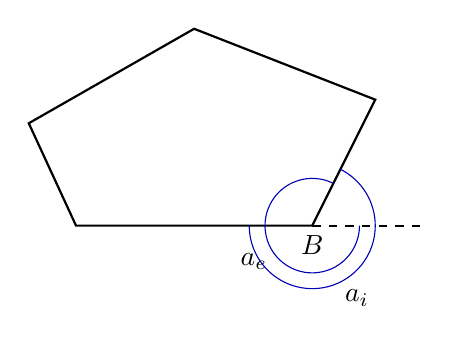
\begin{tikzpicture}[scale=1]
\coordinate (A) at (0,0); \coordinate (B) at (3,0); \coordinate (C) at (3.8,1.6); \coordinate (D) at (1.5,2.5); \coordinate (E) at (-.6,1.3);
\coordinate (X) at (4.4,0);
\draw[thick] (A)--(B)--(C)--(D)--(E)--cycle;
\draw[thick,dashed] (B)--(X);
\pic[draw=blue!70!black, "$a_i$", angle radius=8mm, angle eccentricity=1.35] {angle=A--B--C};
\pic[draw=blue!70!black, "$a_e$", angle radius=6mm, angle eccentricity=1.45] {angle=C--B--X};
\node[below] at (B) {$B$};
\end{tikzpicture}
\hspace{1cm}
% TikZ 4
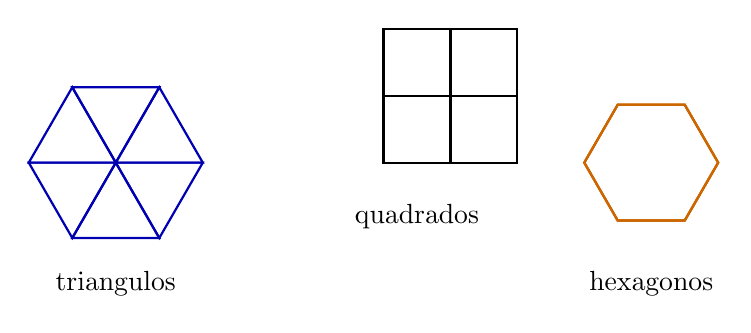
\begin{tikzpicture}[scale=.85]
\foreach \a in {0,60,...,300}{
  \draw[thick,blue!70!black] (0,0)--(\a:1.3)--({\a+60}:1.3)--cycle;
}
\node at (0,-1.8) {triangulos};
\foreach \x/\y in {4/0,5/0,4/1,5/1}{
  \draw[thick] (\x,\y) rectangle +(1,1);
}
\node at (4.5,-.8) {quadrados};
\foreach \a in {0,120,240}{
  \draw[thick,orange!80!black] ({8+cos(\a)},{sin(\a)}) -- ({8+cos(\a+60)},{sin(\a+60)}) -- ({8+cos(\a+120)},{sin(\a+120)}) -- ({8+cos(\a+180)},{sin(\a+180)}) -- ({8+cos(\a+240)},{sin(\a+240)}) -- ({8+cos(\a+300)},{sin(\a+300)}) -- cycle;
}
\node at (8,-1.8) {hexagonos};
\end{tikzpicture}
\end{document}
